\section{Implementação no Arduino}

\begin{frame}{O que é o Arduino?}
  \begin{columns}
    \column{0.6\textwidth}
    O Arduino é uma plataforma prototipagem amplamente utilizada por programadores devido ao seu baixo custo e facilidade para desenvolver \parencite{hughes_2016}. Entre as placas mais populares, destaca-se o Arduino UNO, a escolhida para esse trabalho.
    \begin{table}
      \centering
      \begin{tabular}{cc}
        \hline
        \textbf{Memória Flash} & \textbf{Memória RAM} \\ \hline
        32 kilobytes           & 2 kilobytes          \\ \hline
      \end{tabular}
      \caption{Memória disponível no Arduíno UNO.}
    \end{table}
    \column{0.4\textwidth}
    \begin{figure}
      \centering
      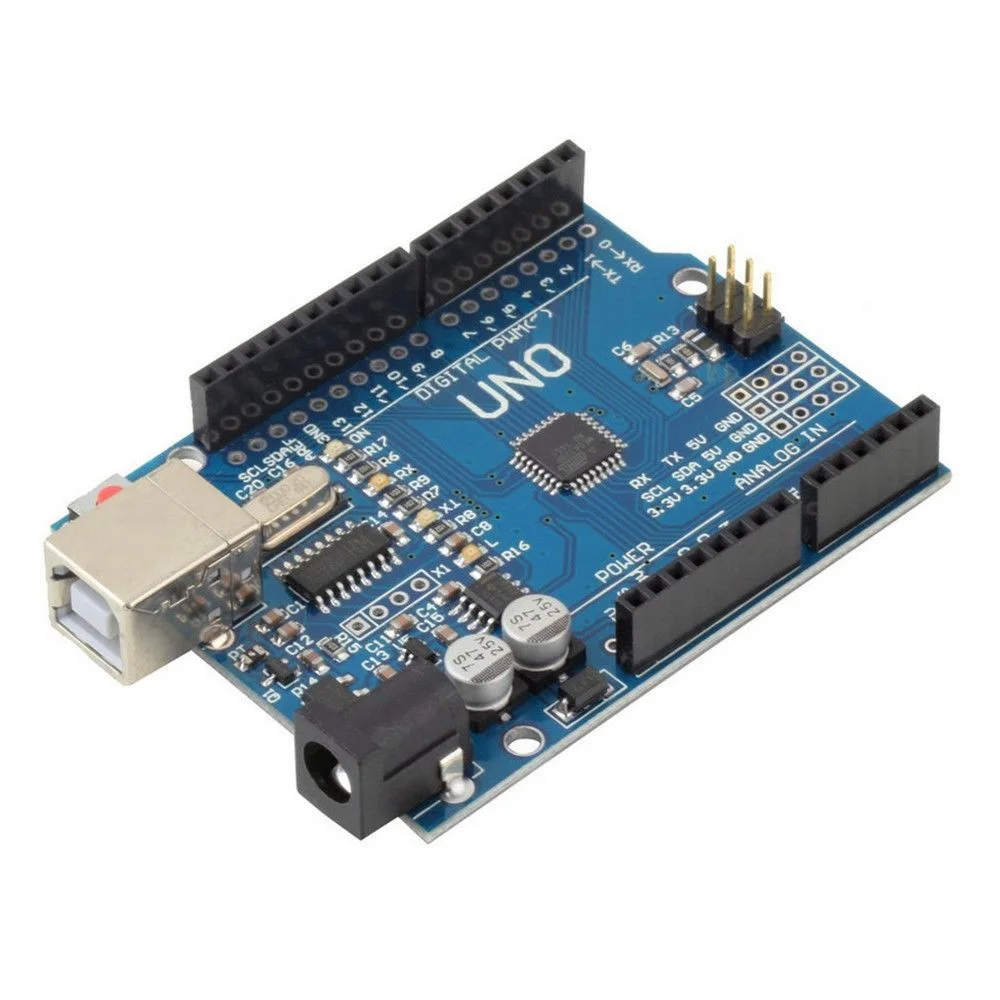
\includegraphics[width=\textwidth]{arduino.png}
      \caption{Placa Arduino UNO. Fonte: makerhero.com}
    \end{figure}
  \end{columns}
\end{frame}

\begin{frame}{O \textit{TankSim}}
  \begin{columns}
    \column{0.6\textwidth}
    \begin{figure}
      \centering
      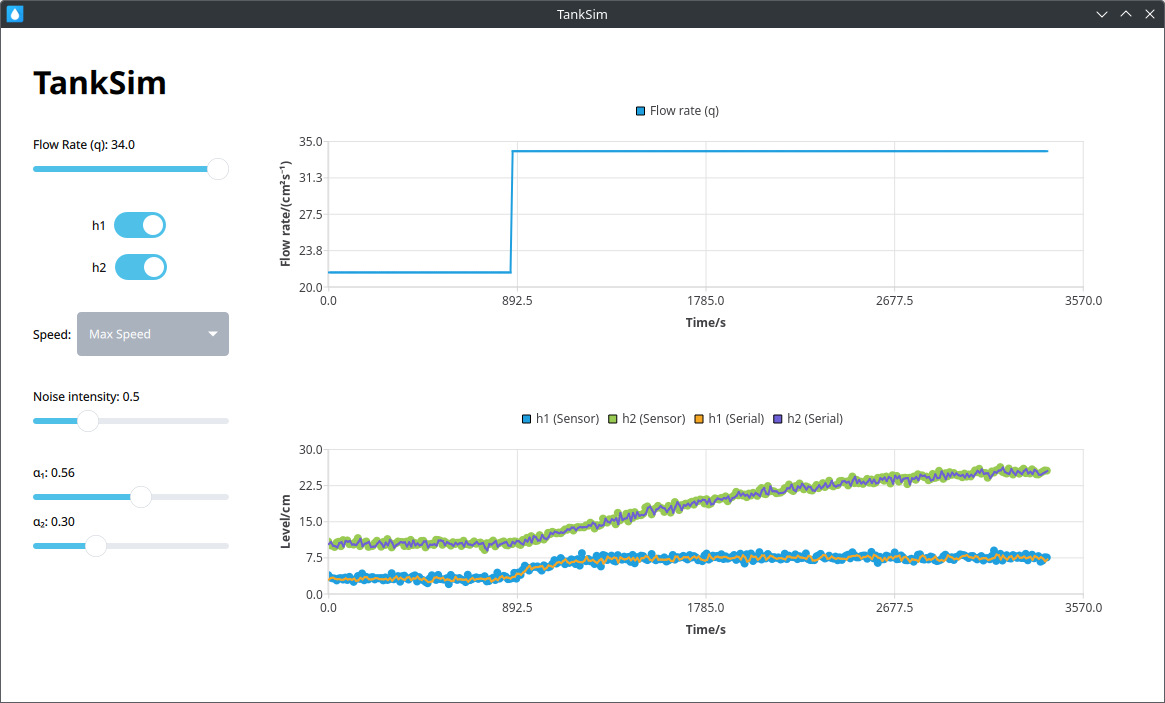
\includegraphics[width=\textwidth]{tanksim.png}
      \caption{Captura de tela do \textit{TankSim}.}
    \end{figure}

    \column{0.4\textwidth}
    O software \textit{TankSim} foi desenvolvido para:
    \begin{itemize}
      \item simular e manipular o funcionamento de uma planta;
      \item realizar a comunicação com o Arduino;
      \item visualizar os valores previstos pela rede neural;
    \end{itemize}
  \end{columns}
\end{frame}

\begin{frame}
  \begin{figure}
    \centering
    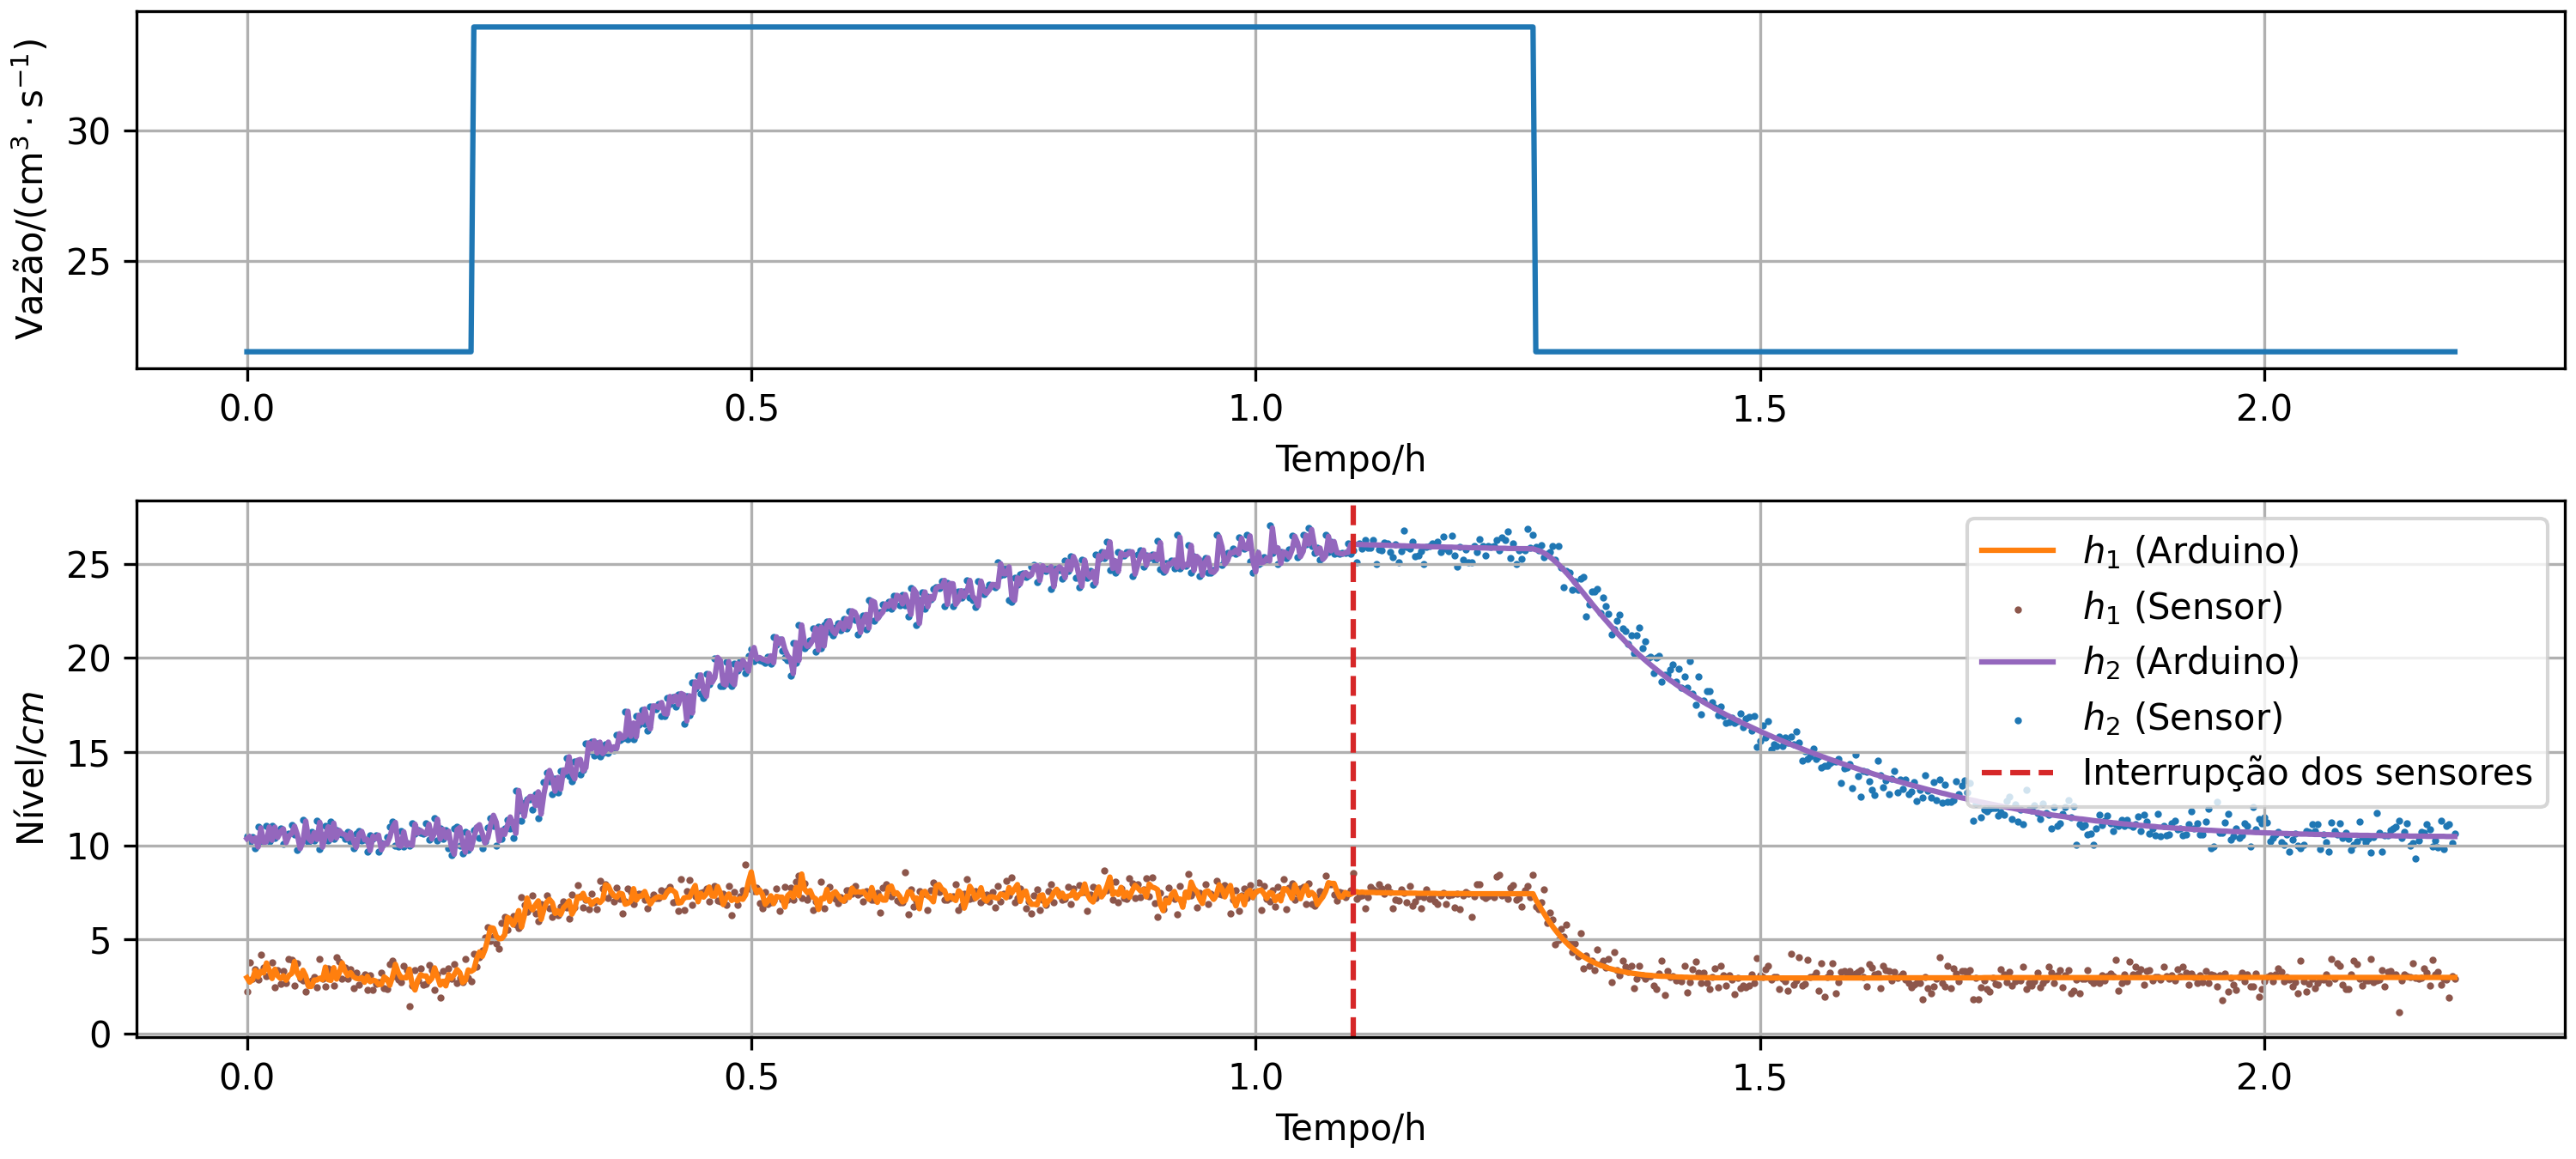
\includegraphics[width=0.9\textwidth]{sil-pirnn.png}
    \caption{Vazão de entrada $q_{\text{in}}$ e nível dos tanques $h_1$ e $h_2$, previstos pelo simulador e pela PIRNN embarcada no Arduino.}
  \end{figure}
\end{frame}